\documentclass[10pt]{article}

% [H] option for figure
\usepackage{graphicx}
\usepackage{float}

%hyper link need to place after graphicx package
\usepackage{hyperref}
\hypersetup{
    colorlinks=true,
    linkcolor=blue,
    filecolor=magenta,      
    urlcolor=cyan,
    citecolor=red,
}




% paragraph spacing
\setlength{\parskip}{0.2em}

% section fontsize
\usepackage{sectsty}
\sectionfont{\fontsize{12}{15}\selectfont}

% margin
\usepackage{geometry}
\geometry{a4paper, portrait, margin=2cm}

% Set column width
\usepackage{array}
\newcolumntype{L}[1]{>{\raggedright\let\newline\\\arraybackslash\hspace{0pt}}m{#1}}
\newcolumntype{C}[1]{>{\centering\let\newline\\\arraybackslash\hspace{0pt}}m{#1}}
\newcolumntype{R}[1]{>{\raggedleft\let\newline\\\arraybackslash\hspace{0pt}}m{#1}}

\begin{document}
%%---------------------------------------
% Title
%---------------------------------------
\noindent
\begin{tabular}{lll R{8.0cm}}
\textbf{Members:} & \textbf{Taimoor Tariq}      & \textbf{20174577} & \textbf{Neural network EE538}\\
\textbf{}         & \textbf{Juan Luis Gonzalez} & \textbf{20178196} & \textbf{Project proposal}\\
\textbf{}         & \textbf{Thang Vu}           & \textbf{20174587} & \textbf{1/Nov/2017}
\end{tabular}\\
\rule[2ex]{\textwidth}{2pt}

%\vspace{0.5cm}
{\Large\centerline{\textbf{Video Super-Resolution Using Convolutional Neural Networks}}}

%%----------------------------------------
% Content
%%----------------------------------------
\section{Goal} % (fold)
\label{sec:goal}
Video Super Resolution (VSR) has remained a challenging problem although some improvement is obtained in recent years. In this project, our goal to design an improved algorithm and network architecture to address this problem. Our model will be compared to the current state-of-the-art, and it is expected that we will obtain better accuracy. 
% section goal (end)

\section{Background} % (fold)
\label{sec:background}
Super Resolution (SR) is the enhancement of image/video resolution. Although SR is a classical problem, it is inherently ill-posed as there are many possibilities to recover for a given low-resolution frame. Typically, SR algorithms can be divided roughly into two categories, which are model-based and learning-based algorithms. Model-based algorithms such as Baysesian approaches have been used for a long time, but with the advent of Deep Learning and Convolutional Neural Networks (CNN), there is great potential for learning-based approaches for image/video super resolution.

\noindent
Image super resolution using CNN has been a topic of a great amount of research in recent years. In theory, CNN is able to learning a non-linear mapping from input to output, producing high-resolution mappings of low-resolution input \cite{dong2016image}. Some methods use input images of smaller sizes and learn mappings to high resolution, whereas other techniques first make use of bicubic interpolation to scale the image then use CNN to improve resolution \cite{dong2016image}. SRCNN is the first model that prove the efficiency of CNN in recovering resolution for single image \cite{dong2016image}. Figure \ref{fig:1} shows an insight on how CNN based image resolution is performed. The SRCNN architecture constitute of three convolutional layers. For a given low-resolution image, the first layer extract the feature maps, then they are map to those of the high-resolution images at the second layer before being reconstructed at the third layer. 

\begin{figure}[H]
    \centering
    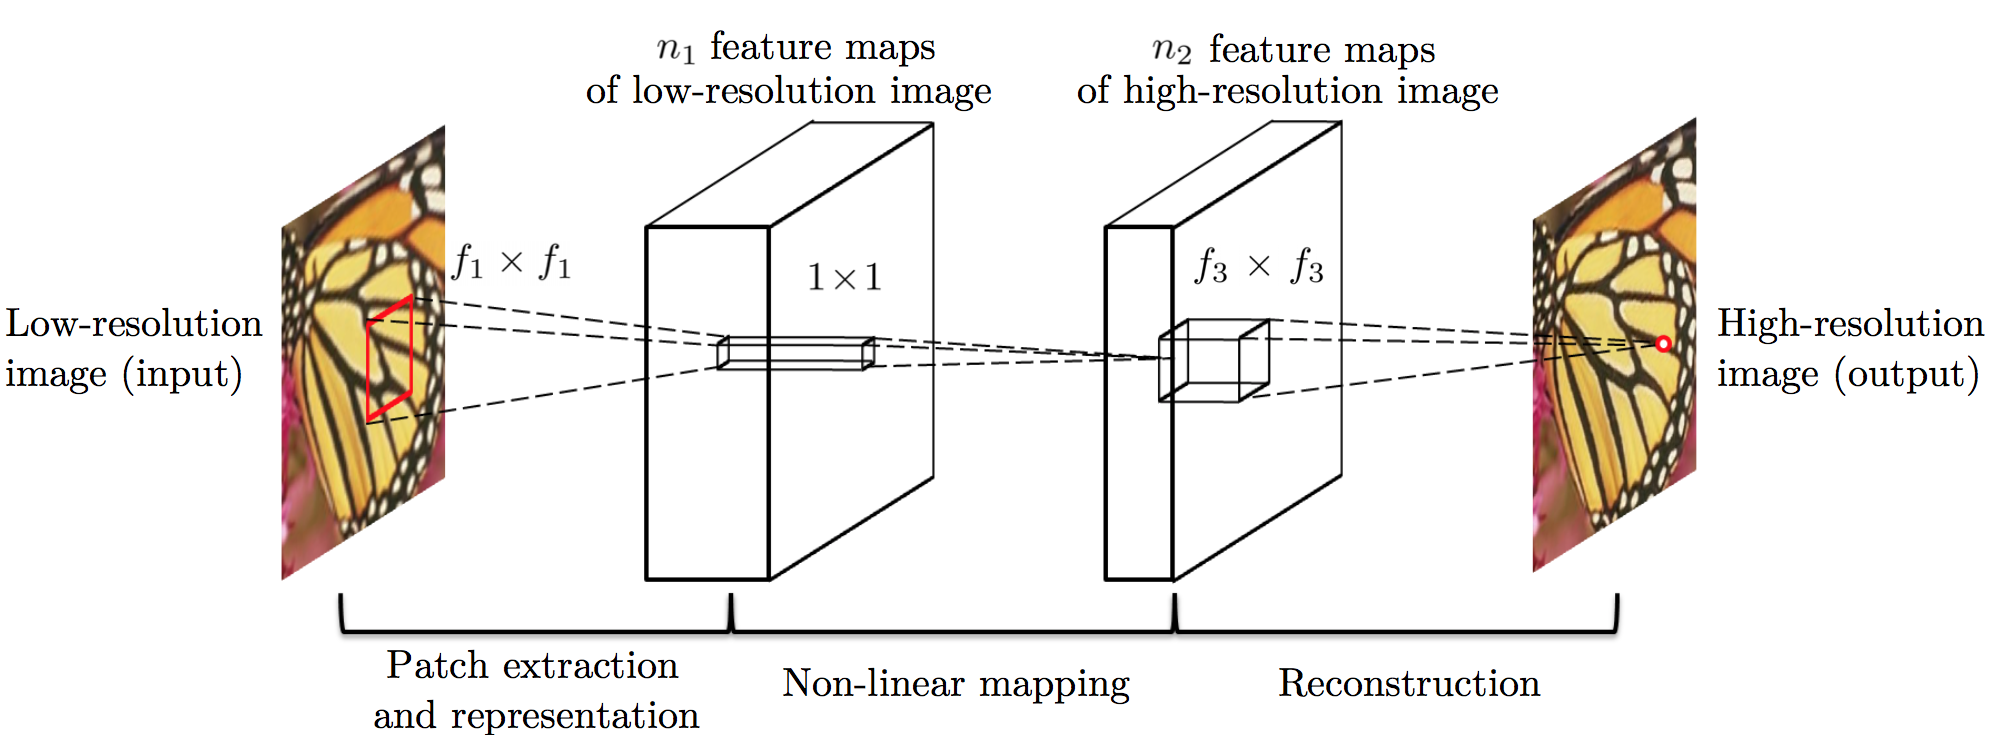
\includegraphics[scale=0.35]{figs/cnn.png}
    \caption{SRCNN architecture for image super resolution}
    \label{fig:1}
\end{figure}

\noindent
Video or multi-frame super resolution(MFSR) has not made nearly as much progress as single-image super resolution. The reason for the difference is that videos have some spatio-temporal relationships between successive frames that can be used to get even better results than image super resolution. These spatio-temporal relationships can be represented in terms of optical flow vector between frames. Existing architectures have been inefficient in harnessing these relationships to produce precision architectures \cite{caballero2016real}. In short, alignment of successive frames in an issue. Motion compensation is a frame alignment technique, which makes use of optical flow vectors to increase correlation among successive frames. Previously, motion compensation was done using methods such as Lucas-Kanade, Horn-Shunk or Bayesian modeling using Gibbs Random Functions. Recently, CNN has been used for motion compensation between frame [NEED CITE HERE]. Some architectures have been proposed that make use of motion compensation and input of many frames. For example, in \cite{greavesmulti}, A. Greaves et. al using the $z$ previous and $z$ next frames to produce high-resolution output with motion compensation (Figure \ref{fig:2}). However, these have been proven to not generalize well and be in consistent \cite{tao2017detail}. Some sub-pixel convolution techniques have been proprosed, but they do not handle occlusion and aperture \cite{shi2016real}.

\begin{figure}[H]
	\centering
	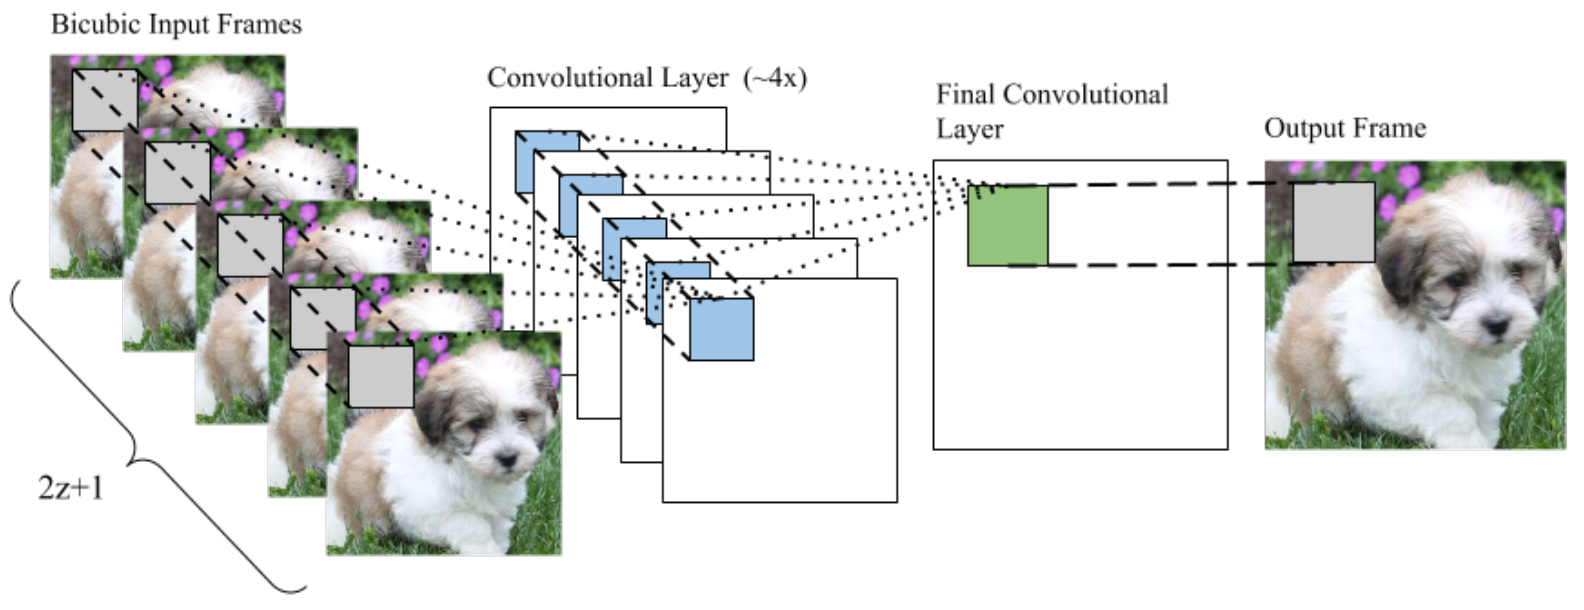
\includegraphics[scale=0.3]{figs/videoCNN.PNG}
	\caption{MFCNN architecture with motion compensation for successive frames}
	\label{fig:2}
\end{figure}

\noindent
The problem of video super resolution using deep learning still has ample potential for investigation. Latest advancements in CNN architectures for computer vision, such as residual deep networks \cite{he2016deep} and dropout can be viable for a more accurate super resolution architecture. 
% section background (end)

\section{Project scope} % (fold)
\label{sec:project_scope}
The first task would be to finalize a system flow, a representation of how the algorithm will probably work. As motion compensated input frames have to be input into the network, we have to finalize an optical flow estimation technique. The technique needs to be robust and relatively immune to issues such as occlusion and aperture. The number of successive frames that need to be input also needs to be investigated. The next step is selection of a network architecture. As residual network have shown good performance for other computer vision tasks, we will try this architecture to see whether the output quality is enhanced or not. Most of the important information is captured in the reference frame, so it needs to be propagated forward. An architecture named MC-SRCNN has been proposed for image super resolution, which used different interpolated forms of the image as input and gives high-resolution output \cite{youm2016image}. This could possibly to be extended to Video super resolution by using different interpolated forms for each input fram and its neighbors. The cost function being used is generally MSE between recovered output and the ground truth. We expect to incorporate PSNR and cross-entropy to ogive a more robust cost function. Another intersting thing that we expect to investigate is the use of Human visual system based Quality metrics (HVS) for cost functions. A new proposed HVS based metric called SC-QI \cite{bae2016novel} is very promising. As we have discussed earlier, the generalization of SR network is a big issue, we will also look at different regularization techniques, even use a combination of them so that the system might give a better performance in a wide variety of scenarios. We will be uing YUV videos for our project, the processing will primarily be done on the Y frames. To evaluate the performance of the model, and compare to some existing methods, PSNR might be used. It is expected to measure the methods with different metrics, but it might depend on our time budget. 
% section project_scope (end)

\section{Schedule plan} % (fold)
\label{sec:schedule_plane}

Table \ref{t:1} describes the schedule for doing the project consisting of 7 main tasks within approximately 8 weeks. For now, we have just finished the proposal, discussed what the challenges of super resolution are, clarified the direction for our project. For the following 2 weeks, we will do literature review. My group has three members so each one takes responsibility on reviewing 2 methods. We will try to answer: "What is new idea for this method? How/Why the method works? What is the limitation of the method". After each paper review, there will be a group meeting to share the knowledge with the other members. Next, we will reproduce the results of the surveyed methods. It is expected to obtain the same results with the authors'. We will do some modifications to make the codes runnable in the same context (test-bed), and we will try to implement the methods that source code is not available. After working on literature review and result reproducing, we will focus on our proposed method. From the related work, it is expected that we will come up with new ideas that extend the existing methods or address their drawbacks. We will focus on network architecture and cost function formulation. For the next week, we will work on model tuning and regularization, and we expect the model will generalize well and be consistent. To have elaborate experiments, we will produce the result of the methods in different setting. Finally, the last 5 days are devoted for the report and presentation.

\noindent
To improve teamwork quality, all the documents for the project will be uploaded into Google Drive folder at the link \url{https://drive.google.com/open?id=0B22Qrl9Ar7OgV08tNzctQkVTSnc}. For implementation, the source code will be available at Github \url{https://github.com/thangvubk/NeuralNetworkProject.git}. 
\begin{table}[H]
\centering
\caption{Schedule plan for the project}
\label{t:1}
\setlength{\tabcolsep}{0.5em} % for the horizontal padding
{\renewcommand{\arraystretch}{2}% for the vertical padding
	\begin{tabular}{L{4cm}ccL{5cm}}
	\hline
	\textbf{Work item}                         & \textbf{Time}   & \textbf{Duration} & \textbf{Notation}                              \\ \hline
	Make proposal                              & 26/Oct - 2/Nov  & 1 week            & \textbf{}                                      \\ \hline
	Literature review                          & 3/Nov - 16/Nov  & 2 weeks           & Try to understand the insight into each method \\ \hline
	Result reproducing                         & 17/Nov - 30/Nov & 2 weeks           & Implement if the source codes are not available \\ \hline
	Propose network architecture and implement & 1/Dec - 7/Dec  & 1 week            &                                                \\ \hline
	Model tuning and regularization            & 8/Dec - 14/Dec  & 1 week            &                                                \\ \hline
	Produce result in different metrics        & 14/Dec - 17/Dec & 4 days            &                                                \\ \hline
	Write final report and make presentation   & 18/Dec - 22/Dec & 5 days            &                                                \\ \hline
	\end{tabular}
}
\end{table}
% section schedule_plane (end)

\section{Expected results} % (fold)
\label{sec:expected_results}
First we will investigate the integrity of our method, as shown in Figure \ref{fig:3}. It is expected that the average PSNR increase as a function of the number of epochs. We will try to make the model generalize well, so that the average testing PSNR should be close to the training value.

\noindent
We also compares our method and some existing methods in term of PSNR and some other metrics if possible. We expect our method will outperform the others or at least be competitive. The result representation will be similar to Figure \ref{fig:4}, which is used to compare SRCNN \cite{dong2016image} to the existing method. For visualization, the results will be described similar to those in Figure \ref{fig:5}

\noindent
For result reproducing, the source code will be public. 
\begin{figure}[H]
	\centering
	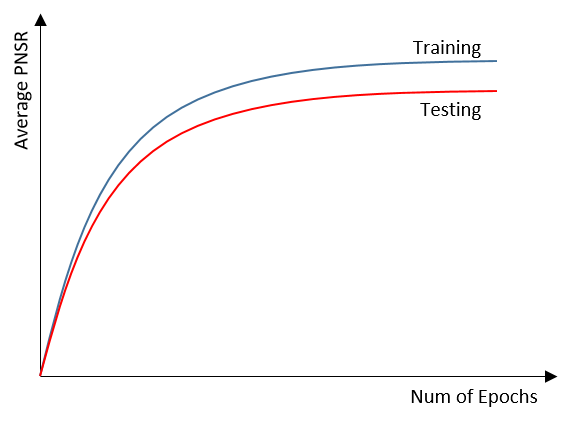
\includegraphics[scale=0.9]{figs/expectedPSNR.png}
	\caption{Expected average training and testing PSNR for the proposed model}
	\label{fig:3}
\end{figure}


\begin{figure}[H]
	\centering
	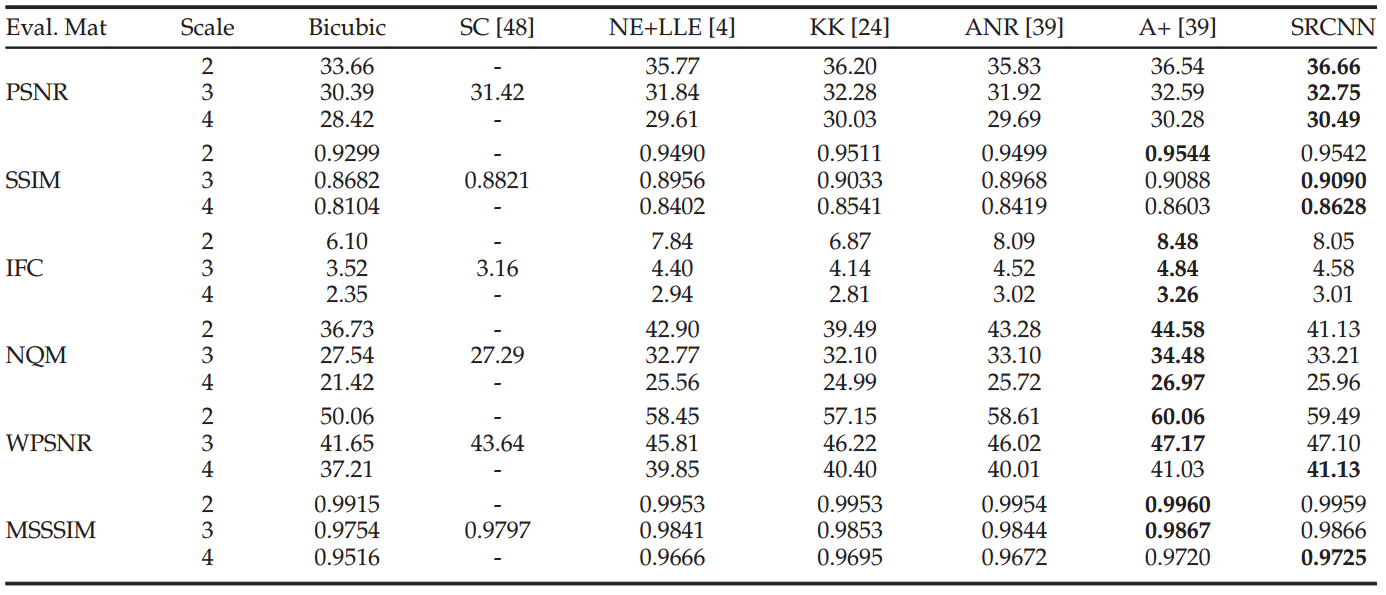
\includegraphics[scale=0.4]{figs/PSNR_table.png}
	\caption{Compare SRCNN and the other method in different metrics}
	\label{fig:4}
\end{figure}

\begin{figure}[H]
	\centering
	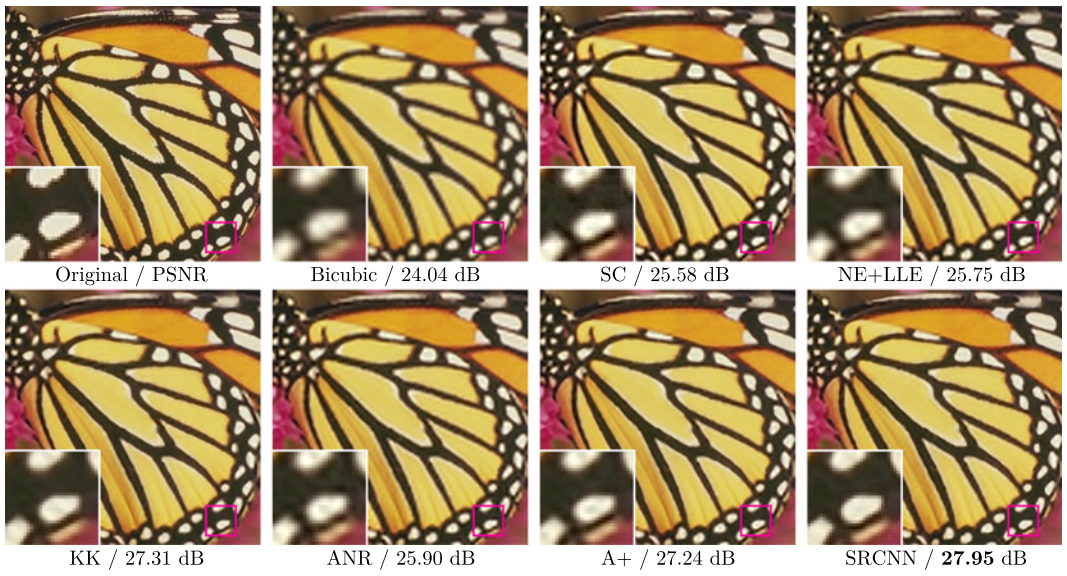
\includegraphics[scale=0.4]{figs/comparePSNR.PNG}
	\caption{PSNR and visualization among the methods}
	\label{fig:5}
\end{figure}

% section expected_results (end)

% References
\bibliographystyle{IEEEtran}
\bibliography{refs}
\end{document}
